\documentclass[11pt]{report}
\usepackage[utf8]{inputenc}
\usepackage[english]{babel}
\usepackage{graphicx}
\usepackage{fancyhdr}
\usepackage{color}
\usepackage{url}
\usepackage{fullpage}

\title{\huge{A Brief Tutorial on FreeRTOS} \\ and its port on the WSN430 hardware platform}
\author{Clément Burin des Roziers}

\begin{document}
   \maketitle

\abstract{This document presents a short introduction to the embedded real-time operating system FreeRTOS, how to port it on the WSN430 hardware platform, and gives some program examples easying the understanding of its features. This is by no mean a complete documentation on FreeRTOS. Such a document may be found on its official website : \url{http://www.freertos.org}}

   \tableofcontents

\chapter{Main Features of FreeRTOS}

FreeRTOS is a lightweight embeddable multi-task real-ime operating system. The produced kernel may require only a few kB of ROM and even less of RAM on the target microcontrolers, hence it is adapted for constrained embedded systems. The kernel source is developed in C language, thus reuse of existing C source code may be easily integrated. As a real-time OS, FreeRTOS focuses on multi-task scheduling and offers the following features:
\begin{itemize}
  \item cooperative, preemptive and hybrid scheduling;
  \item use of tasks and/or co-routines;
  \item multiple inter-tasks communication schemes (queues, semaphores, mutexes).
\end{itemize}

We will describe in deeper details these features now.

\section{Scheduling Modes}
The scheduling works with priorities. The running process will always be the one available with the highest priority. There are two scheduling schemes that may be implemented.
The first is preemptive, which means that a running process may be interrupted to let an other one be executed. The second is cooperative, which means that each process decides where in its execution it may be interrupted. When a process change is to be made, the scheduler chooses the one with the highest priority amongst those ready.

\section{Task Functionality}
A task is a process with its context. Therefore, several tasks can coexist in an application, but do not interfere with each other, they're independent. Since only one task can execute at a time, that is using the CPU, the scheduler swaps in and out the different tasks according to their priorities and the scheduling mode. A task states block diagram may be found in Fig.~\ref{task_diagram}.

\begin{figure}
\begin{center}
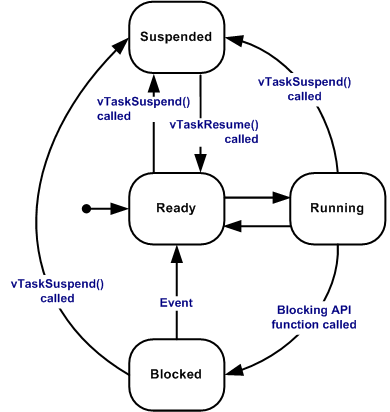
\includegraphics[scale=0.5]{figures/tskstate.png}
\end{center}
\caption{Task States Diagram}
\label{task_diagram}
\end{figure}

A task may be in different states. Here is a brief description of these states:
\begin{description}
	\item[Ready:] a task is ready when it just waits for the scheduler to give it access to the CPU, which means another task with higher or equal priority is running.
	\item[Running:] a task that is actually executing.
	\item[Blocked:] a task that waits for an event before continuing its execution. Events may be temporal (delay) or external (user interaction).
	\item[Suspended:] a task that has been removed from the scheduler. It will not be executed until it's put back to the Ready state.
\end{description}

The task priority is used by the scheduler to define which task to execute (put in the Running state). When several tasks are in the Ready state, it chooses the one with the highest priority. A task with a lower priority than another one will have to wait until this one enters the Blocked state to be executed.

A task is implemented as a function containing an infinite loop. This function should never returns.

There is a task that is systematically created in every application: the idle task. Defined with the lowest priority, it will be executed only when there is no other task in the Ready state. It is possible to define a function that will be called every time the idle task is entered (the idle task hook), which may be interesting for putting the device in a low power mode.

\section{Co-routine Functionality}
Co-routines are a different type of process that may be used for a real time application. The main differences with tasks are that co-routines use prioritized cooperative scheduling, which means they decide when another co-routine may be executed and they share a single stack which reduces the global RAM usage, but requires some special care. Their states diagram is found in Fig.~\ref{cr_diagram}.

\begin{figure}
\begin{center}
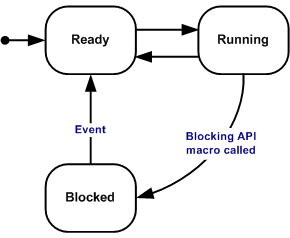
\includegraphics[scale=0.5]{figures/crstate.png}
\end{center}
\caption{Co-routine States Diagram}
\label{cr_diagram}
\end{figure}

A co-routine may be in the following states:
\begin{description}
	\item[Ready:] another co-routine or a task is Running.
	\item[Running:] the co-routine is executing.
	\item[Blocked:] the co-routine is waiting for an event to be Ready again.
\end{description}

The co-routines of an application are prioritized, that is when the scheduler have to choose a co-routine to execute it will take the one in the Ready state with the highest priority. When tasks and co-routines are use simultaneously in an application, any task will always take priority over co-routines. 

\section{Intertask Communication}
\subsection{Queues}

\subsection{Semaphores}
\subsection{Mutexes}


\chapter{Porting FreeRTOS on WSN430 hardware platform}
Download the latest archive from \url{www.freertos.org} and extract it. The FreeRTOS source files organization is as follows: there are two important folders. One is 'Source', it contains the four common files to every architecture with their headers, and the 'portable' folder containing processor specific ports. The other, Demo, contains examples programs for a lot of hardware platforms.

There exists a port of FreeRTOS for the msp430f449 microcontroller on some hardware platform. Thus a few modifications need to be done in order to port it for the WSN430 platform. The port specific source files located in  the 'Source/portable/GCC/MSP430F449' directory are completely compatible with the msp430f1611. Since it is easier to use it directly without renaming it, that's what we'll do. The code in this folders contain processor specific functions (such as configuration of the timer responsible for the scheduler tick interrupt.

We are now going to port the demo application to the WSN430 platform. Copy now the folder 'Demo/msp430\_GCC' to 'Demo/WSN430\_GCC'. There are a few files in it: main.c is the main source code that contains the main function. That's where the tasks will be created and the scheduler started. The file 'FreeRTOSConfig.h' contains a lot of configurations fields allowing the user to specify the characteristics of the kernel. Must be specified the speed of the main clock, the desired tick rate, the available memory on the target and the maximum number of priorities for example. Finally the file 'makefile' contains the compiling directives.

The two directories 'ParTest' and 'serial' contain code for the demo application allowing to control the LEDs and a serial communication respectively. In our first tiny program, we won't need them, they can be deleted. (For information, the target board of the initial port didn't have LEDs but some LCD segments. It is more time consuming to adapt all the existing functions that to rewrite them)

\begin{description}
  \item[FreeRTOSConfig.h] the included header (\#include <msp430x44x.h>) at the top of the file is not for the same msp430. For simplicity, it may be replaced by \#include <io.h>. Next the CPU clock frequency contained in the field configCPU\_CLOCK\_HZ should be updated to 8000000 (8MHz). The tick rate is set to 1000Hz, which is fine, and the heap size may be updated for the new msp430, that is 9800 bytes (out of 10kB RAM).

  \item[makefile] Here we need to update the mmcu used by the compiler by replacing '-mmcu= msp430x449' with '-mmcu= msp430x1611' in the CFLAGS line. We don't have to do the same for the PORT\_PATH line by replacing MSP430F449 since we saw above that the included source files works for both architectures. Finally in the SRC list, we'll need just the minimal, hence we can remove the lines corresponding to ParTest, serial, flash, integer, comtest and PollQ.

  \item[main.c] In the main file, the easiest is to erase everything and start from scratch. We'll go from top to bottom. The required includes are :
\begin{verbatim}
/* Scheduler includes. */
#include "FreeRTOS.h"
#include "task.h"
\end{verbatim}

Then we need some 'define' for simple LEDs handling:
\begin{verbatim}
/* LEDs config */
#define mainLED_TASK_PRIORITY (tskIDLE_PRIORITY + 1)
#define LED_OUT   P5OUT
#define BIT_BLUE   (1 << 6)
#define BIT_GREEN  (1 << 5)
#define BIT_RED    (1 << 4)
\end{verbatim}

Then the file's prototypes:
\begin{verbatim}
/* 
 * The LEDs flashing tasks
 */ 
static void vTaskLED0( void *pvParameters );
static void vTaskLED1( void *pvParameters );
static void vTaskLED2( void *pvParameters );
/*
 * Perform Hardware initialization.
 */
static void prvSetupHardware( void );

\end{verbatim}
And the main function:
\begin{verbatim}
int main( void )
{
  /* Setup the hardware ready for the demo. */
  prvSetupHardware();
  
  /* Start the LEDs tasks  */
  xTaskCreate( vTaskLED0, "LED0", configMINIMAL_STACK_SIZE, \
     NULL, mainLED_TASK_PRIORITY, NULL );
  xTaskCreate( vTaskLED1, "LED1", configMINIMAL_STACK_SIZE, \
     NULL, mainLED_TASK_PRIORITY, NULL );
  xTaskCreate( vTaskLED2, "LED2", configMINIMAL_STACK_SIZE, \
     NULL, mainLED_TASK_PRIORITY, NULL );

  /* Start the scheduler. */
  vTaskStartScheduler();

  /* As the scheduler has been started the demo application
  tasks will be executing and we should never get here! */
  return 0;
}
\end{verbatim}

We have now to develop the task functions:
\begin{verbatim}
/* First LED flash task */
static void vTaskLED0( void *pvParameters )
{
  while (1)
  {
    /* Toggle blue LED and wait 500 ticks */
    LED_OUT ^= BIT_BLUE;
    vTaskDelay(500);
  }
}

/* Second LED flash task */
static void vTaskLED1( void *pvParameters )
{
  while (1)
  {
    /* Toggle green LED and wait 1000 ticks */
    LED_OUT ^= BIT_GREEN;
    vTaskDelay(1000);
  }
}

/* Third LED flash task */
static void vTaskLED2( void *pvParameters )
{
  while (1)
  {
    /* Toggle red LED and wait 2000 ticks */
    LED_OUT ^= BIT_RED;
    vTaskDelay(2000);
  }
}
\end{verbatim}

And finally the hardware setup function:
\begin{verbatim}
static void prvSetupHardware( void )
{
  /* Stop the watchdog timer. */
  WDTCTL = WDTPW + WDTHOLD;

  /* Setup MCLK 8MHz and SMCLK 1MHz */
  DCOCTL  = 0;
  BCSCTL1 = 0;
  BCSCTL2 = SELM_2 | (SELS | DIVS_3) ;

  /* Wait for cristal to stabilize */
  int i;
  do {
    /* Clear OSCFault flag  */
  	IFG1 &= ~OFIFG;
    /* Time for flag to set */
  	for (i = 0xff; i > 0; i--) nop();
  } while ((IFG1 & OFIFG) != 0);

  /* Configure IO for LED use */
  P5SEL  &= ~(BIT_BLUE | BIT_GREEN | BIT_RED);
  P5OUT  &= ~(BIT_BLUE | BIT_GREEN | BIT_RED);
  P5DIR  |=  (BIT_BLUE | BIT_GREEN | BIT_RED);
}
\end{verbatim}

\end{description}

That's it! Now you should be able to compile and load the program to the target, assuming required software (mspgcc) and hardware (JTAG FET) are installed and working.
The three LEDs should be blinking at different rates!


\chapter{Program examples}
\end{document}
